%%%%%%%%%%%%%%%%%%%%%%%%%%%%%%%%%%%%%%%%%%%%%%
%                insertmeeting
% 1) Title (something creative & funny?)
% 2) Date (MM/DD/YYYY)
% 3) Location (ex. Hagerty High School)
% 4) People/Committees Present 
% 5) Picture 
% 6) Start Time & Stop Time (ex. 12:30AM to 4:30PM)
%%%%%%%%%%%%%%%%%%%%%%%%%%%%%%%%%%%%%%%%%%%%%%
\insertmeeting 
	{Wile E Coyote and the Road Runner} 
	{01/05/22} 
	{Hagerty High School}
	{Ritam, James, Nathan, Samantha}
	{Images/RobotPics/robot.jpg}
	{2:30 - 4:30}
	
\hhscommittee{Software}
\noindent\hfil\rule{\textwidth}{.4pt}\hfil
\subsubsection*{Goals}
\begin{itemize}
    \item Read and understand Road Runner and the underlying system for integration to our tricycle drive 

\end{itemize} 

\noindent\hfil\rule{\textwidth}{.4pt}\hfil

\subsubsection*{Accomplishments}
The first resource we found to understand Road Runner was the website "learnroadrunner.com", written by other FTC participants. The main problem we faced was that guide didn't specifically cover a tricycle drive. Most of the guide was written with holonomic drivetrains in mind. However, we did learn a few key points. Because our robot was too narrow to fit 3 dead wheels for localization, we would be forced into using wheel encoders to localize. A consideration for this approach is the possibility of wheel slippage. In theory, slight errors in measurement could cascade into our robot being completely off from where it predicts itself to be. However, we decided to still test the system, as it's possible the slippage is negligible in practice. We also learned about Road Runner's localization system, where they expect the x-axis to be parallel to the red alliance wall. This means that if we have to build our own custom localizer, we must account for difference in coordinate systems between our existing libraries and Road Runner. We also spent some time reading through the usage of Road Runner, including its TrajectoryBuilder system and the tools included. One of the most powerful tools in Road Runner is the ability to quickly create splines, or smooth curves between points. The attached pictures show robot movement with and without the use of splines. It should help us move much more smoothly across the field, increasing our movement efficiency. With this better understanding of Road Runner's capabilities, we can begin integrating their systems into our robot. 
 

\begin{figure}[ht]
\centering
\begin{minipage}[b]{.48\textwidth}
  \centering
  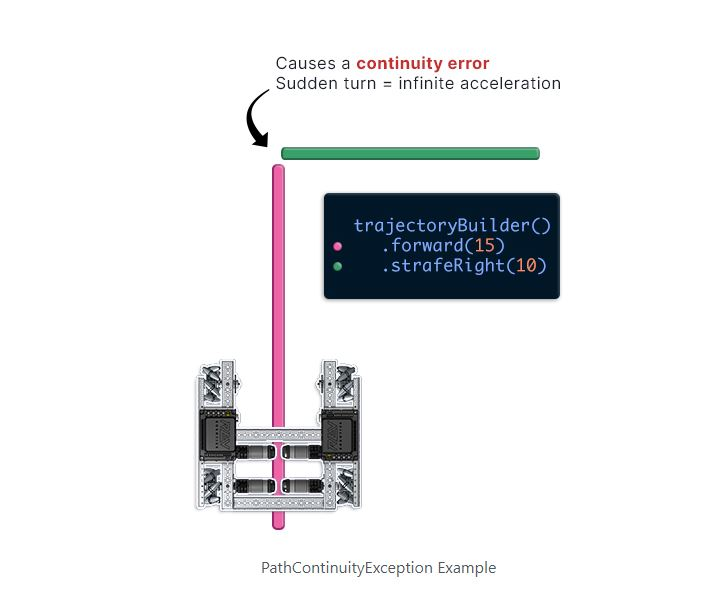
\includegraphics[width=0.95\textwidth]{Meetings/January/01-05-22/1.5.22 without spline - James Hu.JPG}
  \caption{Path we would have to take without using splines and calculations}
  \label{fig:010522_1}
\end{minipage}%
\hfill%
\begin{minipage}[b]{.48\textwidth}
  \centering
  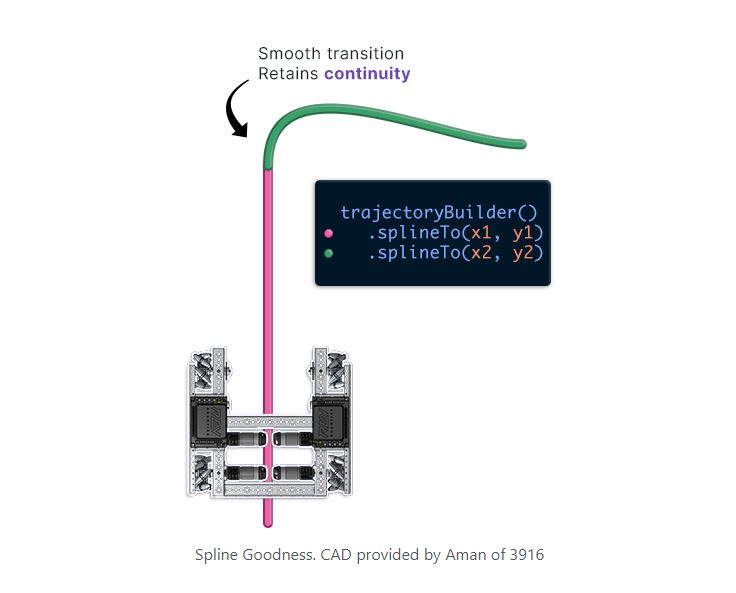
\includegraphics[width=0.95\textwidth]{Meetings/January/01-05-22/1.5.22 with spline - James Hu.JPG}
  \caption{What we can do with Road Runner}
  \label{fig:010522_2}
\end{minipage}
\end{figure}


\hhscommittee{Multimedia}
\noindent\hfil\rule{\textwidth}{.4pt}\hfil
\subsubsection*{Goals}
\begin{itemize}
    \item Our goal for today's meeting is to establish a more detailed Promote Video storyboard that described the who, what, and where of each main scene. 

\end{itemize} 

\noindent\hfil\rule{\textwidth}{.4pt}\hfil

\subsubsection*{Accomplishments}An important aspect of our Promote video is to keep it psychologically engaging. In other words, we want people to be left thinking about the storyline to the point where they feel the need to replay it. To do this, we structured the plot to be a loop, where it could be replayed and the storyline would continue to make sense. To do so, we had to innovate what phrases would begin and end the script. We did this by coming up with phrases that we liked and wanted to include, then highlighting them in different colors based on which part of the script it would occur during. For today, our committee only completed the main phrases "So if there was only one thing I could tell my younger self, it would be" and "take the wheel", but have rough ideas down for the scenes in between.
 


\whatsnext{
\begin{itemize}
    \item Next meeting will be for solidifying more of the script and loop idea.
\end{itemize} 
}

